%% Start of file `dndicons.tex`.
%% Copyright 2024 Jasper Habicht (mail@jasperhabicht.de).
%
% This work may be distributed and/or modified under the
% conditions of the LaTeX Project Public License version 1.3c,
% available at http://www.latex-project.org/lppl/.

\documentclass{ltxdoc}
\def\dndiconsfileversion{1.3.1}
\def\dndiconsfiledate{18 February 2024}

\usepackage[T1]{fontenc}
\usepackage{longtable, booktabs}
\usepackage[pics]{dndicons}

\EnableCrossrefs
\CodelineIndex
\RecordChanges

\RenewDocumentCommand{\PrintMacroName}{ m }{
 \color{red}
}

\NewDocumentEnvironment{dndiconsexamplecolumn}{ O{0.4} }{%
    \noindent%
    \begin{minipage}[t]{#1\linewidth}%
    \vspace{0pt}%
}{ 
    \vspace{0pt}%
    \end{minipage}
}

\NewDocumentEnvironment{dndiconsiconlist}{ }{
    \begin{longtable}{ @{} p{17em} p{3em} p{\dimexpr\linewidth-20em-4\tabcolsep} @{} }
    \toprule
    \textbf{Command} & \textbf{Icon} & \textbf{Shape} \\ 
    \midrule\endhead
}{
    \bottomrule
    \end{longtable}
}

\NewExpandableDocumentCommand{\dndiconsiconlistentry}{ m }{
    \multicolumn{3}{ @{} l @{} }{#1}
}

\begin{document}

\title{The \texttt{dndicons} package \\[5pt] \Large A set of high quality icons made with Ti\emph{k}Z for use in notes for tabletop role-playing games}
\author{Jasper Habicht\thanks{E-mail: \href{mailto:mail@jasperhabicht.de}{mail@jasperhabicht.de}}}
\date{Version \dndiconsfileversion, released on \dndiconsfiledate}

\maketitle

\changes{v1.1.0}{2023/08/15}{First public release.}
\changes{v1.1.1}{2023/11/15}{Fudge dice icon added.}
\changes{v1.1.2}{2023/11/16}{Bug fixed that caused wrong spacing when using dice icons without quantifier.}
\changes{v1.2.0}{2023/11/20}{Corrections in the manual. Icons for six-sided dice with one to nine pips, plus sign and minus sign added.}
\changes{v1.2.1}{2023/11/20}{Documentation of lengths for spacing added.}
\changes{v1.2.2}{2023/11/21}{Corrections in the manual.}
\changes{v1.3.0}{2023/11/21}{Option to set background color added. Renamed global option.}
\changes{v1.3.1}{2024/02/18}{Correction of initializing code. Correction of default value of after sep. Addition of pics.}

\bigskip

\section{Introduction}

The \verb+dndicons+ package provides a set of high quality icons made with Ti\emph{k}Z for use in notes for tabletop role-playing games. The icons are meant to be used in the body text, but they can also be used in other contexts such as graphics or diagrams.

Since the commands to typeset the icons typeset \verb+tikzpicture+ environments, these commands should not be used inside another \verb+tikzpicture+. However, because the package defines the icons as Ti\emph{k}Z shapes, it is possible to use the icons in \verb+tikzpicture+ environments directly. Apart from that, as of version 1.1.0, the package provides a way to define custom commands to typeset the icons as boxed material which is safe to use in a \verb+tikzpicture+ context.

\section{Loading the package}

The \verb+dndicons+ package is loaded by calling \verb+\usepackage{dndicons}+ in the preamble of the document. 

\begin{macro}{pics}
The package provides the option \verb+pics+. If the package is loaded with this option, every icon is also available as Ti\emph{k}Z pic. On the use of pics, see section \ref{sec:pics} below.
\end{macro}

\subsection{Dependencies}

The package loads the \verb+tikz+ package which in turn loads the \verb+xcolor+ package. If you want to make use of certain options these packages provide, you need to load the packages with the relevant options beforehand or use, for example, \verb+\PassOptionsToPackage{svgnames}{xcolor}+.

\section{Usage}

Once loaded, the package provides a set of commands that can be used to print icons inline. The package also defines a set of node shapes that can be used inside a \verb+tikzpicture+ environment. 

\subsection{Global settings}

\begin{macro}{dnd icons}
All icons share the Ti\emph{k}Z style \verb+dnd icons+ that has no options per default but can be used to style all icons at once. For example, if the setting \verb+\tikzset{dnd icons/.append style={draw=red}}+ is placed at the beginning of the document, all icons will be drawn in red. Per default, the icons are drawn in the color of the surrounding text. 

Note that it may be necessary to add the Ti\emph{k}Z option \verb+transform shape+ when applying transformations to the icons, because the icons are realised as Ti\emph{k}Z nodes which are not affected by some transformations per default.
\end{macro}

\begin{macro}{dnd icons/background color}
In most cases, the icons are made of drawn paths. However, some icons can be used with a negative color scheme where the icon is drawn negatively inside a filled shape. Per default, the icons are drawn in white in such cases, but it might be desirable that the icons are in the same color as the background. To this end, the color can be changed using the Ti\emph{k}Z option \verb+dnd icons/background color+ in the following way:
\end{macro}

\begin{dndiconsexamplecolumn}%
    \colorbox{blue!50}{%
        \ability[negative]{charisma}
            [scale=2, transform shape]%
    }
    
    \tikzset{
        dnd icons/background color={blue!50}
    }
    \colorbox{blue!50}{%
        \ability[negative]{charisma}
            [scale=2, transform shape]%
    }
\end{dndiconsexamplecolumn}%
\begin{dndiconsexamplecolumn}[0.4]%
\begin{verbatim}
\colorbox{blue!50}{%
    \ability[negative]{charisma}
        [scale=2, transform shape]%
}

\tikzset{
    dnd icons/background color={blue!50}
}
\colorbox{blue!50}{%
    \ability[negative]{charisma}
        [scale=2, transform shape]%
}
\end{verbatim}%
\end{dndiconsexamplecolumn}

This feature can, of course, also be used to change the color of the icon independently from the color of the background.

\begin{macro}{dnd icons/before sep, dnd icons/after sep}
The Ti\emph{k}Z optins \verb+dnd icons/before sep+ and \verb+dnd icons/after sep+ are used to define the width of the space that is added before and after the icons respectively. The default value of both lengths is 0.05\,em. For example, setting the space before icons to 1\,cm can be achieved as follows:
\end{macro}

\begin{dndiconsexamplecolumn}%
    Roll\die{eightside}{}a die!
    
    \tikzset{
        dnd icons/before sep={1cm}
    }
    Roll\die{eightside}{}a die!
\end{dndiconsexamplecolumn}%
\begin{dndiconsexamplecolumn}[0.6]%
    \begin{verbatim}
Roll\die{eightside}{}a die!

\tikzset{
    dnd icons/before sep={1cm}
}
Roll\die{eightside}{}a die!
    \end{verbatim}%
\end{dndiconsexamplecolumn}

\subsection{Icons}

Because the package defines the icons as Ti\emph{k}Z shapes, every command can actually be used together with every shape. However, the combinations of shapes and commands as described in the following subsections are preferable.

\subsubsection[Icon \textbackslash die]{Icon \cmd{\die}}

\begin{macro}{\die}
The command \cmd{\die}\oarg{style}\marg{shape}\oarg{options}\marg{integer} prints an icon to depict a die with a certain number of sides. Two special icons exist for a two-sided die (which would be equivalent to a coin) and for a hundred-sided die (which typically comes in the shape of a sphere). There is also a special icon for a fudge die. 

For the six-sided die, nine additional shapes exists representing the values one to nine as pips. Also, additional shapes exist representing the plus or minus side of a fudge die.

The command takes two mandatory commands, the first of which describes the shape (see previous subsection) and the second can take an integer that is placed in front of the shape. Thus, \verb+\die{eightside}{2}+ results in \die{eightside}{2} (meaning 2 eight-sided dice are rolled).

The command also takes two optional arguments, the second of which can take arbitrary Ti\emph{k}Z options to style the icon. The options affect the shape, not the integer when it is printed before the icon. As an example, \verb+\die{eightside}[blue, thick]{2}+ results in \die{eightside}[blue, thick]{2}.

The first optional argument can take the value \verb+normal+ or \verb+large+, \verb+normal+ being the default value. With \verb+large+ given as argument, the icon is drawn larger and the additional integer is printed inside of the shape instead of before it. As an example, \verb+\die[large]{eightside}{2}+ results in \die[large]{eightside}{2}. Note that the integer will always be printed on top of the shape, even if the shape does not have an open center as in the case of the \verb+fudge+ shapes or the shapes featuring pips. 
\end{macro}

\begin{dndiconsiconlist}
\dndiconsiconlistentry{\cmd{\die}\oarg{style}\marg{shape}\oarg{options}\marg{integer}} \\
    & \die{twoside}{} & \verb+twoside+ \\
    & \die{fourside}{} & \verb+fourside+ \\
    & \die{sixside}{} & \verb+sixside+ \\
    & \die{eightside}{} & \verb+eightside+ \\
    & \die{tenside}{} & \verb+tenside+ \\
    & \die{twelveside}{} & \verb+twelveside+ \\
    & \die{twentyside}{} & \verb+twentyside+ \\
    & \die{hundredside}{} & \verb+hundredside+ \\
    & \die{fudge}{} & \verb+fudge+ \\
    & \die{sixside one}{} & \verb+sixside one+ \\
    & \die{sixside two}{} & \verb+sixside two+ \\
    & \die{sixside three}{} & \verb+sixside three+ \\
    & \die{sixside four}{} & \verb+sixside four+ \\
    & \die{sixside five}{} & \verb+sixside five+ \\
    & \die{sixside six}{} & \verb+sixside six+ \\
    & \die{sixside seven}{} & \verb+sixside seven+ \\
    & \die{sixside eight}{} & \verb+sixside eight+ \\
    & \die{sixside nine}{} & \verb+sixside nine+ \\
    & \die{fudge plus}{} & \verb+fudge plus+ \\
    & \die{fudge minus}{} & \verb+fudge minus+ \\
\end{dndiconsiconlist}

\subsubsection[Icons \textbackslash ability and \textbackslash saving]{Icons \cmd{\ability} and \cmd{\saving}}

\begin{macro}{\ability}
The command \cmd{\ability}\oarg{style}\marg{shape}\oarg{options} prints icons depicting an ability of a character. The abilities are represented by animal-like shapes. The relevant shape should be given as mandatory argument to the command. The second optional argument can take arbitrary Ti\emph{k}Z options to style the icon.

The first optional argument can take the value \verb+positive+ or \verb+negative+, \verb+positive+ being the default value. With \verb+negative+ given as argument, the icon is drawn negative inside a circle. As an example, \verb+\ability[negative]{charisma}+ results in \ability[negative]{charisma}.
\end{macro}

\begin{macro}{\saving}
The command \cmd{\saving}\oarg{style}\marg{shape}\oarg{options} prints the icons that can be typeset using the \cmd{\ability} command inside a small shield. It can take the same values for the mandatory argument as the \cmd{\ability} command. The optional argument can take arbitrary Ti\emph{k}Z options to style the icon.

The first optional argument can take the value \verb+normal+ or \verb+empty+, \verb+normal+ being the default value. With \verb+empty+ given as argument, the icon inside the shield is not printed. In this case, the mandatory argument can be left empty. As an example, \verb+\saving[empty]{}+ results in \saving[empty]{}. 
\end{macro}

\begin{dndiconsiconlist}
\dndiconsiconlistentry{\cmd{\ability}\oarg{style}\marg{shape}\oarg{options}} \\
    & \ability{strength} & \verb+strength+ \\
    & \ability{dexterity} & \verb+dexterity+ \\
    & \ability{dexterity alt} & \verb+dexterity alt+ \\
    & \ability{constitution} & \verb+constitution+ \\
    & \ability{intelligence} & \verb+intelligence+ \\
    & \ability{wisdom} & \verb+wisdom+ \\
    & \ability{charisma} & \verb+charisma+ \\
    & \ability{luck} & \verb+luck+ \\
    & \ability{armor} & \verb+armor+ \\
    & \ability{proficiency} & \verb+proficiency+ \\
\midrule
\dndiconsiconlistentry{\cmd{\saving}\marg{shape}\oarg{options}} \\
    & \saving{strength} & \verb+strength+ \\
    & \saving{dexterity} & \verb+dexterity+ \\
    & \saving{dexterity alt} & \verb+dexterity alt+ \\
    & \saving{constitution} & \verb+constitution+ \\
    & \saving{intelligence} & \verb+intelligence+ \\
    & \saving{wisdom} & \verb+wisdom+ \\
    & \saving{charisma} & \verb+charisma+ \\
    & \saving{luck} & \verb+luck+ \\
    & \saving{armor} & \verb+armor+ \\
    & \saving{proficiency} & \verb+proficiency+ \\
\end{dndiconsiconlist}

\subsubsection[Icon \textbackslash spell]{Icon \cmd{\spell}}

\begin{macro}{\spell}
The command \cmd{\spell}\marg{shape}\oarg{options} prints icons depicting the effect of a spell or how it is to be effected. The optional argument can take arbitrary Ti\emph{k}Z options to style the icon.
\end{macro}

\begin{dndiconsiconlist}
\dndiconsiconlistentry{\cmd{\spell}\marg{shape}\oarg{options}} \\
    & \spell{linear} & \verb+linear+ \\
    & \spell{conic} & \verb+conic+ \\
    & \spell{quadratic} & \verb+quadratic+ \\
    & \spell{cubic} & \verb+cubic+ \\
    & \spell{spheric} & \verb+spheric+ \\
    & \spell{cylindric} & \verb+cylindric+ \\
    & \spell{verbal} & \verb+verbal+ \\
    & \spell{somatic} & \verb+somatic+ \\
    & \spell{material} & \verb+material+ \\
    & \spell{focus} & \verb+focus+ \\
\end{dndiconsiconlist}

\subsubsection[Icon \textbackslash spellschool]{Icon \cmd{\spellschool}}

\begin{macro}{\spellschool}
The command \cmd{\spellschool}\oarg{style}\marg{shape}\oarg{options} prints icons that represent the school a spell belongs to. The second optional argument can take arbitrary Ti\emph{k}Z options to style the icon.

The first optional argument can take the value \verb+negative+ or \verb+positive+, \verb+negative+ being the default value. Per default the icon is drawn in white inside a filled escutcheon. With \verb+positive+ given as argument, the icon as well as the escutcheon are drawn in the currently selected color. As an example, \verb+\spellschool[positive]{evocation}+ results in \spellschool[positive]{evocation}.
\end{macro}

\begin{dndiconsiconlist}
\dndiconsiconlistentry{\cmd{\spellschool}\oarg{style}\marg{shape}\oarg{options}} \\
    & \spellschool{abjuration} & \verb+abjuration+ \\
    & \spellschool{conjuration} & \verb+conjuration+ \\
    & \spellschool{divination} & \verb+divination+ \\
    & \spellschool{enchantment} & \verb+enchantment+ \\
    & \spellschool{evocation} & \verb+evocation+ \\
    & \spellschool{illusion} & \verb+illusion+ \\
    & \spellschool{necromancy} & \verb+necromancy+ \\
    & \spellschool{transmutation} & \verb+transmutation+ \\
\end{dndiconsiconlist}

\subsubsection[Icons \textbackslash damage, \textbackslash attack, and \textbackslash condition]{Icons \cmd{\damage}, \cmd{\attack}, and \cmd{\condition}}

\begin{macro}{\damage}
The command \cmd{\damage}\marg{shape}\oarg{options} prints icons depicting the damage of an attack. The icon is printed inside a circle. The optional argument can take arbitrary Ti\emph{k}Z options to style the icon.
\end{macro}

\begin{macro}{\attack}
The command \cmd{\attack}\marg{shape}\oarg{options} prints icons depicting the kind of an attack. The optional argument can take arbitrary Ti\emph{k}Z options to style the icon.
\end{macro}

\begin{macro}{\condition}
The command \cmd{\condition}\marg{shape}\oarg{options} prints icons depicting a condition of a character. The optional argument can take arbitrary Ti\emph{k}Z options to style the icon.
\end{macro}

\begin{dndiconsiconlist}
\dndiconsiconlistentry{\cmd{\damage}\marg{shape}\oarg{options}} \\
    & \damage{acid} & \verb+acid+ \\
    & \damage{bludgeoning} & \verb+bludgeoning+ \\
    & \damage{cold} & \verb+cold+ \\
    & \damage{fire} & \verb+fire+ \\
    & \damage{force} & \verb+force+ \\
    & \damage{lightning} & \verb+lightning+ \\
    & \damage{necrotic} & \verb+necrotic+ \\
    & \damage{piercing} & \verb+piercing+ \\
    & \damage{poison} & \verb+poison+ \\
    & \damage{psychic} & \verb+psychic+ \\
    & \damage{radiant} & \verb+radiant+ \\
    & \damage{slashing} & \verb+slashing+ \\
    & \damage{thunder} & \verb+thunder+ \\
    & \damage{healing} & \verb+healing+ \\
\midrule
\dndiconsiconlistentry{\cmd{\attack}\marg{shape}\oarg{options}} \\
    & \attack{melee} & \verb+melee+ \\
    & \attack{ranged} & \verb+ranged+ \\
    & \attack{magic} & \verb+magic+ \\
    & \attack{singlehanded} & \verb+singlehanded+ \\
    & \attack{doublehanded} & \verb+doublehanded+ \\
\midrule
\dndiconsiconlistentry{\cmd{\condition}\marg{shape}\oarg{options}} \\
    & \condition{buff} & \verb+buff+ \\
    & \condition{blinded} & \verb+blinded+ \\
    & \condition{charmed} & \verb+charmed+ \\
    & \condition{deafened} & \verb+deafened+ \\
    & \condition{exhausted} & \verb+exhausted+ \\
    & \condition{frightened} & \verb+frightened+ \\
    & \condition{grappled} & \verb+grappled+ \\
    & \condition{incapacitated} & \verb+incapacitated+ \\
    & \condition{invisible} & \verb+invisible+ \\
    & \condition{paralyzed} & \verb+paralyzed+ \\
    & \condition{petrified} & \verb+petrified+ \\
    & \condition{poisoned} & \verb+poisoned+ \\
    & \condition{prone} & \verb+prone+ \\
    & \condition{restrained} & \verb+restrained+ \\
    & \condition{stunned} & \verb+stunned+ \\
    & \condition{unconscious} & \verb+unconscious+ \\
    & \condition{hearing} & \verb+hearing+ \\
    & \condition{seeing} & \verb+seeing+ \\
\end{dndiconsiconlist}

\subsection{Direct use of shapes}

Because the icons are defined as Ti\emph{k}Z shapes, they can directly be applied to Ti\emph{k}Z nodes. However, the shapes don't have a shape border and no anchors except for the \verb+center+ anchor that sits exactly in the center of the shape. Therefore, if nodes with these shapes are connected using edges, the \verb+center+ anchor will be used to connect the nodes. If nodes with these shapes are being positioned, only the \verb+center+ anchor is available. Text content of these nodes is simply printed on top of the center of the node. Compare the following example.

\begin{dndiconsexamplecolumn}%
    \begin{tikzpicture}
        \node[eightside, blue, thick] at (0,0) (A) {A};
        \node[charisma] at (2,0) (B) {B};
        \draw[red] (A) -- (B);
    \end{tikzpicture}
\end{dndiconsexamplecolumn}%
\begin{dndiconsexamplecolumn}[0.6]%
    \begin{verbatim}
\begin{tikzpicture}
    \node[eightside, blue, thick] 
        at (0,0) (A) {A};
    \node[charisma] at (2,0) (B) {B};
    \draw[red] (A) -- (B);
\end{tikzpicture}
    \end{verbatim}%
\end{dndiconsexamplecolumn}

\subsection{Icons as pics}\label{sec:pics}

If the package is loaded with the option \verb+pics+, every icon is also available as Ti\emph{k}Z pic. The names of the pic always start with \verb+dnd icons+ followed by a space and the name of the relevant icon (see the lists above). For abilities, savings, spellschools and damages, additional pics exists where the name has the suffixes \verb+ability+, \verb+saving+, \verb+spellschool+, and \verb+damage+ respectively.

The icon is embedded as a node in the pic which has the name \verb+-node+. Thus, it is possible to name the pic and refer to the node inside. Due to the fact that the icon is a node, the option `transform shape` has to be used if transformations on the pic are to affect the node as well. It is easily possible to apply styles to the node using the Ti\emph{k}Z option \verb+every node+ as shown in the following example.

\begin{dndiconsexamplecolumn}%
    \begin{tikzpicture}
    \pic[
        transform shape,
        scale=2, 
        fill=blue, 
        draw=red, 
        every node/.style={
            white,
            thick
        }
    ] (p) {dnd icons charisma ability};
    \draw (p-node) -- +(1,-1);
    \end{tikzpicture}
\end{dndiconsexamplecolumn}%
\begin{dndiconsexamplecolumn}[0.6]%
    \begin{verbatim}
\begin{tikzpicture}
    \pic[
        transform shape,
        scale=2, 
        fill=blue, 
        draw=red, 
        every node/.style={
            white,
            thick
        }
    ] (p) {dnd icons charisma ability};
    \draw (p-node) -- +(1,-1);
\end{tikzpicture}
    \end{verbatim}%
\end{dndiconsexamplecolumn}

\NewExpandableDocumentCommand{\ellipsis}{ }{%
    \textcolor{gray}{...} %
}

\begin{macro}{dnd icons/create pic \textcolor{gray}{...}, from shape, 
    from ability shape, 
    from saving shape, 
    from spellschool shape, 
    from damage shape}
The package defines five Ti\emph{k}Z keys that are used to create pics using the relevant node shapes. In normal circumstances, it is not necessary to use these keys. They are mentioned here primarily for reference. 
\end{macro}

\vspace*{3\baselineskip}

\subsection{Boxing of icons}

Because the icons cannot simply be used inside \verb+tikzpicture+ environments, the package provides a workaround to place icons inside of boxes for later use. Icons that are boxed this way can safely used inside \verb+tikzpicture+ environments. This might be necessary, if an icon should be used in inline text that sits inside a node.

\begin{macro}{\provideprotecteddndicon}\sloppy
The command \cmd{\provideprotecteddndicon}\marg{command}\oarg{style}\marg{shape}\oarg{op\-tions}\marg{box name} creates a box containing the icon that would be created using one of the regular commands this package provides. For example, the command \verb+\provideprotecteddndicon{die}[large]{eightside}[blue, thick]{mybox}+ stores the icon of an eight-sided die with the relevant style and Ti\emph{k}Z options in a new box named \verb+mybox+. Note that no integer can be added to the \cmd{\die} command in this context.
\end{macro}

\provideprotecteddndicon{die}[large]{eightside}[blue, thick]{mybox}

\begin{macro}{\useprotecteddndicon}
Using the command \cmd{\useprotecteddndicon}\marg{box name}, the previously defined box can be used to place the relevant icon. With the above definition, \verb+\useprotecteddndicon{mybox}+ would result in \useprotecteddndicon{mybox}.
\end{macro}

Having created a boxed icon, it is safe to use it, for example, inside a Ti\emph{k}Z node:

\begin{dndiconsexamplecolumn}%
    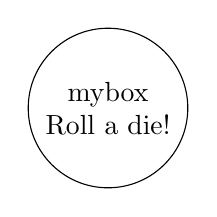
\begin{tikzpicture}
        \node[circle, draw, align=center] {
            \useprotecteddndicon{mybox} \\ 
            Roll a die!
        };
    \end{tikzpicture}
\end{dndiconsexamplecolumn}%
\begin{dndiconsexamplecolumn}[0.6]%
    \begin{verbatim}
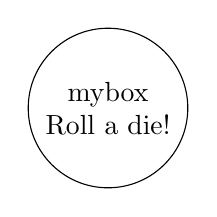
\begin{tikzpicture}
    \node[circle, draw, align=center] {
        \useprotecteddndicon{mybox} \\ 
        Roll a die!
    };
\end{tikzpicture}
    \end{verbatim}%
\end{dndiconsexamplecolumn}

\PrintChanges

\end{document}

%% End of file `dndicons.tex`.
